\section{tasks::getspecshift Class Reference}
\label{classtasks_1_1getspecshift}\index{tasks::getspecshift@{tasks::getspecshift}}
Inheritance diagram for tasks::getspecshift::\begin{figure}[H]
\begin{center}
\leavevmode
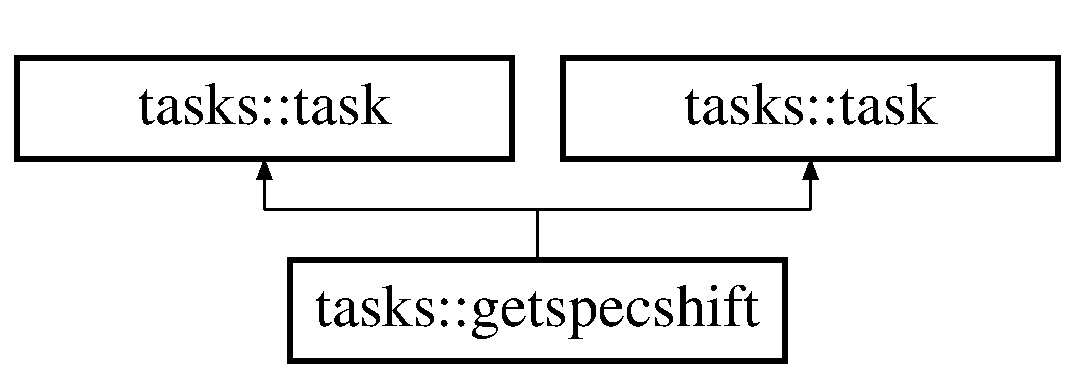
\includegraphics[height=2cm]{classtasks_1_1getspecshift}
\end{center}
\end{figure}
\subsection*{Public Member Functions}
\begin{CompactItemize}
\item 
def \textbf{run}\label{classtasks_1_1getspecshift_9d2c0ae4d503b9ace36fb95efb3c774a}

\item 
def \textbf{run}\label{classtasks_1_1getspecshift_9d2c0ae4d503b9ace36fb95efb3c774a}

\end{CompactItemize}
\subsection*{Static Public Attributes}
\begin{CompactItemize}
\item 
string \textbf{name} = '{\bfgetspecshift}'\label{classtasks_1_1getspecshift_1151b6e77da357b7a8b7ba64357f427c}

\item 
string \textbf{button\-Text} = 'Determine spectrum shift'\label{classtasks_1_1getspecshift_ff492a9ffb50fd1bb4e87dc95e789743}

\item 
string \textbf{suffix} = 'specshift'\label{classtasks_1_1getspecshift_c30c0182aa89a375061e301ffec5ad22}

\item 
list \textbf{prereq} = ['{\bfpreproc}']\label{classtasks_1_1getspecshift_ad17795867562b353e02ea4012a661c8}

\end{CompactItemize}


\subsection{Detailed Description}


\footnotesize\begin{verbatim}Determine the spectrum shift by extracting the interlaced spectrum
   and comparing this to the interlaced wavelength reference frame.
\end{verbatim}
\normalsize
 



The documentation for this class was generated from the following files:\begin{CompactItemize}
\item 
old/PANICtool-1.0/tasks.py\item 
old/tasks.py\end{CompactItemize}
